\documentclass[10pt,a4paper]{article}

\bibliographystyle{ieeetr}

\usepackage[margin=1in]{geometry}
\usepackage{graphicx}
\usepackage{subfig}
\usepackage{amsmath}
\usepackage{url}
\usepackage{pgfgantt}
%\usepackage{diagbox}

\newcommand{\code}[1]{\texttt{#1}}

\title{A modular kernel for the Raspberry Pi: Project Specification}

\begin{document}

\maketitle

\begin{center}
    Thomas Archbold \\
    1602581 \\
    University of Warwick \\
\end{center}

\section*{Background}
In most operating systems, many design decisions are made in order to keep
things simple for the user, by keeping most of the technical details hidden. In
most cases, this is an appropriate approach: needlessly offering more choices
for low-level tasks that are usually handled by the operating system, such as
CPU and disk scheduling algorithms, would only serve to confuse the average
user. It may actually be detrimental to the security and the stability of the
system by opening up more opportunities for errors to be introduced.  This more
insulated approach does mean, however, that the user never really knows what is
going on ``under the hood'', and indeed whether greater performance can be
achieved by making \textit{different} fundamental decisions.  Furthermore, a
number of operating systems exist for the Raspberry Pi, some focusing on
ease-of-installation, others on Internet of Things integration, such as the
NOOBS \cite{NOOBS} Linux distribution or the Windows 10 IoT Core distribution
\cite{IoT}. However, none exist to serve as an experimental operating system,
designed to be a testbed for making and changing these low-level behaviours.
This project aims to fill this gap for the operating systems enthusiast, one who
wishes to test for themselves the different approaches to CPU scheduling, disk
scheduling, interprocess communication, and filesystems. It will give the user
the ability to alter the fundamental ways in which their machine operates by
compiling different modules to handle different tasks, without the need to
reboot, enabling for a more flexible operating system where such things can be
tweaked at any point.

\section*{Main goal}
The goal of this project is to create a modular operating system for the
Raspberry Pi 2 Model B that is capable of loading different modules at
compilation time to tackle CPU scheduling, disk scheduling, interprocess
communication, and filesystems in a variety of ways. Specifically, it must have
some way to run and switch between multiple processes using a CPU scheduler;
interact with a hard disk drive and a disk scheduler for permanent/mass storage;
and be able to create, read, update, and delete files and directories using a
custom filesystem.  To achieve this, it must implement an interface for
loading/removing modules, similar to Linux's \code{insmod} and \code{rmmod}
\cite{insmod}, and must do so safely and stably.  Furthermore, as executing
processes forms a key functional requirement for the project, there must be a
convenient way to load programs into memory and begin their execution. A
solution to both of these problems is to implement a basic shell/command
interpreter.

Finally, a key objective of this project will be to get the operating system to
work entirely on real hardware, and not solely in an emulated environment. This
includes booting from the SD card installed in the Raspberry Pi. As the boot
process is handled by the Pi's System on Chip (SoC), so booting will be possible
without writing a custom bootloader. On top of booting from it, the operating
system must interact with the SD card in conjunction with a filesystem for
permanent/mass storage. Finally, it must be capable of taking input from a
keyboard connected via USB, and printing output to a physical screen via its
HDMI port.

\subsubsection*{Loadable modules}
The project must implement the following as loadable modules, which may be
configured at compilation time by the user:
\begin{itemize}
    \item CPU Scheduling:
        \begin{itemize}
            \item First Come First Served
            \item Round Robin
            \item Shortest Job First
            \item Shortest Remaining Time First
            \item Priority Scheduling (preemptive and non-preemptive)
            \item Lottery Scheduling
        \end{itemize}
    \item Interprocess Communication
        \begin{itemize}
            \item Message passing
            \item Shared memory
        \end{itemize}
    \item Filesystem
        \begin{itemize}
            \item persistent
            \item load-on-request
        \end{itemize}
\end{itemize}

\subsection*{Stretch goals}
Some stretch goals which should be implemented to show understanding of more
complex structures would be some more intricate scheduling algorithms, including
the following \cite{CFS,BFS,DinosaurCPU,O(n)Scheduler,O(1)Scheduler}:
\begin{itemize}
    \item Completely Fair Scheduler
    \item Multiple Queue Skiplist Scheduler, MuQSS
    \item Multilevel Queue and Multilevel Feedback Queue
    \item $\mathcal{O}(n)$ Scheduler
    \item $\mathcal{O}(1)$ Scheduler
\end{itemize}

In order to give the operating system more purpose and to increase usability,
the collection of relatively simple programs on offer should be extended,
including a mix of long running CPU- and I/O-bound programs. This will mean that
the relative performance of the schedulers may be seen more easily. While the
Not Recently Used (NRU) algorithm will be used for page replacement due to its
low overhead and decent performance, other algorithms could be explored and
implemented as modules. These may include: First-In-First-Out (to highlight its
poor performance), the Clock Page Replacement algorithm, and the Least Recently
Used algorithm \cite{PageReplacement}.

\subsection*{Further extensions}
Beyond these goals, further extensions would focus on increasing the usability
of the system, and start to shape it into one which someone might actually use
to get things done. One of the simpler ways to achieve this would be to write a
text editor. Additionally, implementing networking into the operating system
would vastly increase its usability and general usefulness. Such goals are
rather far-fetched given the time frame of the project, but would form
meaningful projects later in the life of the operating system.

\subsection*{Out-of-scope}
Features which will not be implemented in th eproject include graphical user
interfaces and any form of security. Graphics would increase the complexity of
the project too much, and provide too little reward, to be considered a
worthwhile goal. While security would be easier to implement, for example by
following suit of Linux's permissions interface \cite{permissions}, it would
again detract attention from features more in line with the project's goals.
After all, the operating system produced will only be experimental and designed
for use by one user, and as such security will be an unnecessary feature.

\section*{Hardware}
The main reason for choosing to work with the Raspberry Pi was its boot process,
which is detailed below. In particular, as it is handled entirely by its SoC, it
means a custom bootloader capable of loading the kernel into memory and
transferring control to it will need not be written. The motivation behind
opting for the Raspberry Pi 2 Model B specifically was because of its prior
availability to the author, and meant some other model need not be bought when
it came to running on real hardware. The Raspberry Pi 1, 2, and 3 use the
Broadcom BCM2835, BCM2836, and BCM2837 respectively, and the underlying
architecture behind these chips are identical. The only difference from the 2's
chip to the BCM2835 is that the ARM1176JZF-S processor has been replaced with a
quad-core Cortex-A7 cluster \cite{BCM2835}. Similarly, this chip only differs
from the BCM2837 in that this Cortex-A7 cluster is replaced by a quad-core ARM
Cortex A53 (ARMv8) cluster \cite{BCM2837}. This is all to say that the
differences between the different versions of the Pi are likely to be
insignificant when compared with the focus of the project, in that it is
concerned with producing an operating system simply for \textit{some} version of
the Pi.

\begin{center}
    \begin{figure}[h]
        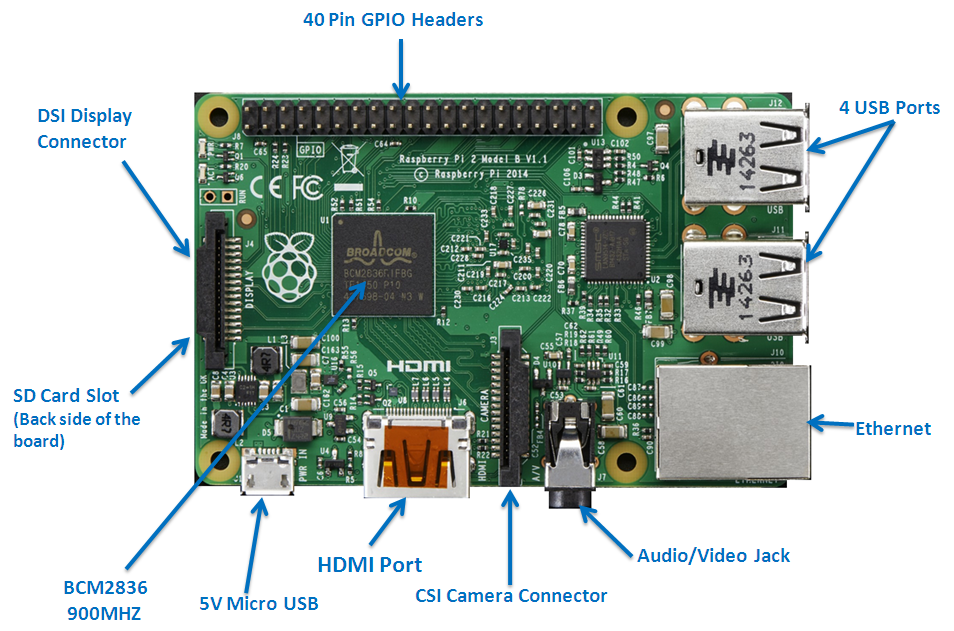
\includegraphics[width=4in]{pi-diagram.png}
        \caption{Raspberry Pi 2 Model B}
    \end{figure}
\end{center}

\subsection*{A note about the Raspberry Pi's boot process}

% Talk about boot process
% diagrams and technical specs

\section*{Methodology}
The methodology best suited to the project will be a mix between a plan-driven
and agile approach; the basic requirements of the system will not change over
the course of the project, and furthermore there will be a rigid structure with
regards to dependencies that the project is likely to abide by (for example, the
system will have to boot before implementing memory management before
implementing scheduling algorithms). Therefore, the early stages of the project
will benefit from a plan driven approach, most likely an Incremental one to
allow for some choice in what to implement, as opposed to the more restrictive
structure of a Waterfall methodology. After the foundations have been
implemented successfully, the project is likely to open up and take a more agile
approach; Scrum cycles are likely to be useful dedicating a large portion of
concentration implementing one feature, or fixing specific bugs, at one time, in
an incremental manner.

Throughout the project, weekly meetings will be held with the supervisor in
order to discuss any current problems and talk through approaches to solutions
(especially for the more complex ones), the overall progress of the project, as
well as the direction in which it is headed. It would also be at this time that
progress is compared with the timetable, and any notes and adjustments are made
dynamically in order to fully stay on top of the work.

\section*{Testing}
The project will be tested in an incremental manner. Especially to begin with,
it is vital that some systems operate correctly before moving on and developing
other areas. As the project progresses and its complexity increases, unit tests
will be written to systematically cover all, or at least most, likely paths of
execution, and to account for each of these. The most fundamental requirement to
fulfill while testing the solution will be stability, that is to say, whether
the system is able to safely switch between different modules and continue
operation. Of course, the solution must also be correct: the user must be able
to switch dynamically between the different modules, and the system must react
accordingly. There must be a way to verify that the system is indeed operating
in the way that is expected from the user, and again, unit tests and
verification software must be produced to ensure this.

\section*{Timetable}
\begin{ganttchart}{1}{12}
    \gantttitle{2011}{12} \\
    \gantttitlelist{1,...,12}{1} \\
    \ganttgroup{Group 1}{1}{7} \\
    \ganttbar{Task 1}{1}{2} \\
    \ganttlinkedbar{Task 2}{3}{7} \ganttnewline
    \ganttmilestone{Milestone}{7} \ganttnewline
    \ganttbar{Final Task}{8}{12}
    \ganttlink{elem2}{elem3}
    \ganttlink{elem3}{elem4}
\end{ganttchart}

\section*{Technologies}
The following technologies will be used by the project:
\begin{itemize}
    \item Git - version control
    \item Github - to access the project from multiple sources, as well as to
        back it up
    \item C - the language in which most of the operating system will be
        implemented
    \item ARM assembly - used when C is unavailable/inappropriate
        \cite{CannotDoC}
    \item GCC cross compiler for ARM EABI - for cross compiling for the target
        processor, the Cortex-A7 \cite{CrossCompilation}
    \item QEMU - for emulating the Pi to allow quicker and safer testing
        \cite{qemu}
    \item Make - used to speed up the build process
\end{itemize}

\section*{Resources}
The following documentation will be used throughout for reference to the
architecture of the Cortex-A7 processor and its intruction set:
        \begin{itemize}
            \item Cortex-A7 MPCore Technical Reference Manual
            \item ARM Cortex-A Series Programmer's Guide
            \item Broadcom BCM2835 ARM Peripherals Manual
        \end{itemize}

\section*{Legal, social, ethical, and professional  considerations}
All software used to build the project is available to use under the GNU Public
License. Throughout the project's development, some testing will be required
from people other than the creator, to gain informal feedback especially with
regards to usability; these people are likely to be friends and colleagues,
hence the social, ethical, and professional issues are insignificant.

\bibliography{bibliography}

\end{document}
